% !TEX program = xelatex
% Standalone CVPR-style supplementary material.
\documentclass[10pt,twocolumn,letterpaper]{article}
\usepackage[review]{cvpr}
% Portable Times-compatible Unicode fonts; CVPR geometry is unchanged.
\usepackage{iftex}
\ifXeTeX
  \usepackage{fontspec}
  \setmainfont{texgyretermes-regular.otf}[
    BoldFont=texgyretermes-bold.otf,ItalicFont=texgyretermes-italic.otf,
    BoldItalicFont=texgyretermes-bolditalic.otf]
  \setsansfont{texgyreheros-regular.otf}[
    BoldFont=texgyreheros-bold.otf,ItalicFont=texgyreheros-italic.otf,
    BoldItalicFont=texgyreheros-bolditalic.otf]
  \setmonofont{texgyrecursor-regular.otf}[
    BoldFont=texgyrecursor-bold.otf,ItalicFont=texgyrecursor-italic.otf,
    BoldItalicFont=texgyrecursor-bolditalic.otf]
\fi

\usepackage{xeCJK}
\setCJKmainfont{FandolSong-Regular.otf}[BoldFont=FandolSong-Bold.otf,ItalicFont=FandolKai-Regular.otf]
\setCJKsansfont{FandolHei-Regular.otf}[BoldFont=FandolHei-Bold.otf]
\setCJKmonofont{FandolFang-Regular.otf}
\usepackage{booktabs}
\usepackage{graphicx,placeins,multirow,float}
\usepackage{amsmath,amssymb}
\definecolor{cvprblue}{rgb}{0.21,0.49,0.74}
\usepackage[pagebackref,breaklinks,colorlinks,allcolors=cvprblue]{hyperref}
\def\paperID{*****}
\def\confName{CVPR}
\def\confYear{2027}
\title{DriveCompose：通过联合补全实现驾驶场景的可组合生成式重建}
\author{Anonymous CVPR Submission}
\begin{document}
% Allow related supplementary result tables to share a page without changing fonts or geometry.
\setcounter{topnumber}{5}
\setcounter{dbltopnumber}{5}
\setcounter{totalnumber}{10}
\renewcommand{\topfraction}{0.9}
\renewcommand{\dbltopfraction}{0.9}
\renewcommand{\textfraction}{0.05}
\renewcommand{\floatpagefraction}{0.75}
\renewcommand{\dblfloatpagefraction}{0.75}
% Keep lineno's column marker before the column contents (legacy wrapper).
% The inherited CVPR style with this TeX version places the hook marker after
% the contents in the standalone supplementary title path.
\makeatletter
\RemoveFromHook{build/column/before}[lineno]
\let\DCoriginalmakecol\@makecol
\def\@makecol{%
  \DCoriginalmakecol
  \setbox\@outputbox\vbox{%
    \boxmaxdepth\@maxdepth
    \protected@write\@auxout{}{%
      \string\def\string\@LN@column{\if@firstcolumn1\else2\fi}}%
    \box\@outputbox}}
\let\@LN@makecol\@makecol
\makeatother

\maketitlesupplementary
\appendix
\renewcommand{\thetable}{S\arabic{table}}
\renewcommand{\theequation}{S\arabic{equation}}
\renewcommand{\thefigure}{S\arabic{figure}}
\section{跨数据集泛化}
\label{sec:generalization}

我们评价从 Waymo 到 nuScenes 的零样本迁移，以考察模型在训练数据集之外的重建质量。将在 Waymo 上训练的检查点直接应用于 nuScenes，评价时固定全部模型参数。

如表~\ref{tab:generalization} 所示，DriveCompose 在所比较方法中取得最高的 PSNR 和 SSIM，分别达到 26.47 dB 和 0.803，比表现最好的基线 DGGT 分别提高 1.16 dB 和 0.009。这些结果表明，在不进行目标域适配的情况下，DriveCompose 提升了目标数据集上的重建质量。

\begin{table}[!htbp]
\centering
\small
\setlength{\tabcolsep}{10pt}
\renewcommand{\arraystretch}{1.08}
\caption{从 Waymo 到 nuScenes 的零样本泛化。PSNR 和 SSIM 越高越好。}
\label{tab:generalization}
\begin{tabular}{@{}lcc@{}}
\toprule
& \multicolumn{2}{c}{Zero-shot} \\
\cmidrule(lr){2-3}
Method & PSNR $\uparrow$ & SSIM $\uparrow$ \\
\midrule
STORM~\cite{yang2025storm} & 17.77 & 0.669 \\
DGGT~\cite{chen2025dggt} & 25.31 & 0.794 \\
StreetForward~\cite{yu2026streetforward} & 23.17 & 0.712 \\
\midrule
Ours & \textbf{26.47} & \textbf{0.803} \\
\bottomrule
\end{tabular}
\end{table}


\section{训练细节}
\label{sec:supp-training}

学习分为四个阶段，使补全目标具有稳定含义。恢复模块确定证据与支撑，编解码器定义潜空间坐标，补全网络学习缺失潜码的分布。最后一个阶段将该分布适配到真实观测，同时保持其预测的表示不变。

\paragraph{数据组成与划分。}
表~\ref{tab:data-splits} 的数量均为质量检查后的有效数据。Waymo 原训练集划分为 740 条训练与 58 条开发序列，开发集用于选模，202 条验证序列用于测试。合成地图、车辆基础模型及人体身份按源资产隔离；同一模型的不同纹理、同一人体的不同服装及动作留在同一划分。真实日志按路段、连续采集片段和可识别身份去重隔离。完整性指有限查询支撑内的几何、材质与运动绑定目标完整性。

\begin{table*}[!t]
\centering\small
\setlength{\tabcolsep}{4pt}
\caption{数据与监督来源。场景地图和独立资产均按源身份划分。}
\label{tab:data-splits}
\begin{tabular}{@{}lrrrp{0.47\textwidth}@{}}
\toprule
数据 & 训练 & 开发 & 测试 & 监督 \\
\midrule
Waymo 序列 & 740 & 58 & 202 & 图像、标定、自车位姿、LiDAR、车辆框与轨迹 \\
自建合成场景 & 10,000 & 1,000 & 1,000 & 完整几何、材质、深度、语义、实例及演员状态 \\
合成场景地图 & 80 & 10 & 10 & 静态背景几何及道路结构 \\
独立车辆资产 & 10,000 & 1,000 & 1,000 & 完整规范几何、材质、尺寸及刚体坐标系 \\
独立人体身份 & 2,500 & 250 & 250 & 身份体型、纹理、规范模板、骨架、蒙皮及关节状态 \\
\bottomrule
\end{tabular}
\end{table*}


\paragraph{固定布局上的完整目标。}
部分输入建立 $\mathcal Q$。两个分支使用相同的查询位置、尺度、类型和顺序，并共享组件归属与人体绑定，沿用 \texttt{QueryBundle.blocks} 的块顺序及块内索引。完整网格沿该固定支撑查询。对非天空查询，将所属组件网格转换到查询坐标系，与支撑单元 $B_i$ 求交；非零面积的相交三角片提供表面目标。资产完整性检查通过且没有相交表面的单元采用无表面目标。

面积为 $A_f$ 的相交三角片 $f$ 采用
\begin{equation}
n_f=\max\!\left(1,\left\lceil\frac{64A_f}{\delta_{\min}^{\,2}}\right\rceil\right)
\label{eq:target-samples}
\end{equation}
个确定性面积样本，$\delta_{\min}$ 为单元最短边。资产、查询和三角片编号共同确定采样位置。在固定照明与原始材质下渲染 RGB、光轴深度、实例及三角片编号。基础视图包含八个方位角和三个仰角，局部隔离视图覆盖剩余相交片，为基础视图中被遮挡的表面提供特征。

阶段一训练后冻结的同一视觉编码器将渲染 RGB 映射为 128 维特征。在各表面样本投影处提取特征，附加相对查询中心的归一化深度残差，并截断至 $[-1,1]$。先在每个样本的有效视图间按观测权重平均，再按相交片面积聚合，形成 $\mathbf h_i^{\rm full}\in\mathbb R^{129}$。部分分支沿用查询中心投影和可见性加权聚合。

无表面单元采用 129 维零特征和明确的零不透明度监督。无表面目标描述网格表面的缺失，自由空间标签来自观测射线。天空目标由完整环境贴图提供，深度残差为零。两分支共享视觉特征基、输入格式和类型专属 codec，目标潜码为
\begin{equation}
\mathbf z_{1,i}=E_{k_i}([\mathbf h_i^{\rm full};\mathbf q_i;\boldsymbol\delta_i])
\in\mathbb R^{128}.
\label{eq:complete-code}
\end{equation}
135 维输入依次通过 $135\rightarrow128\rightarrow128$ MLP 与 LayerNorm。编码器偏置允许零特征映射为非零潜码；补全过程的硬投影另行将自由空间潜码清零。

\begin{table*}[t]
\centering\small
\caption{网络与空间支撑配置。基础网格另保留观测锚点和规范人体模板查询。}
\label{tab:network-config}
\begin{tabular}{@{}lp{0.70\textwidth}@{}}
\toprule
模块 & 配置 \\
\midrule
视觉恢复 & 宽度 128，patch 尺寸 16，4 头；1 层图像注意力和 2 层跨视图／时刻摘要交互 \\
身份与人体状态 & 24 个身份槽，10 维体型码，17 关节接口 \\
查询特征与潜码 & 特征 129 维，潜码 128 维；分类型 $135\rightarrow128\rightarrow128$ 编码器及 LayerNorm \\
补全网络 & 宽度 128，4 层，4 头，16 个记忆 token \\
高斯解码 & 每查询 4 个子高斯，每个 23 个输出参数，其中外观参数 12 个 \\
方向外观 & 每颜色通道包含常数项和三个局部方向系数 \\
基础支撑 & 背景 $20\times12\times6$，刚体 $8\times4\times4$，天空每面 $4\times4$ \\
采样 & 24 步显式 Euler，每步恢复已见潜码并清零自由空间潜码 \\
\bottomrule
\end{tabular}
\end{table*}

\paragraph{阶段一：视觉恢复。}
真实训练日志与合成场景监督图像编码器、几何预测头、身份槽和状态头。真实深度来自训练 LiDAR，车辆状态来自标注；带置信度的真实语义及人体关节辅助标签，与合成体型、骨架、绑定和关节监督共同训练恢复模块。整条轨迹执行一次身份匹配，并在各时刻复用。置信度根据深度、遮挡和重投影可靠性训练或校准，各项权重见表~\ref{tab:recovery-weights}。

\begin{table}[t]
\centering\small
\caption{阶段一监督权重。}
\label{tab:recovery-weights}
\begin{tabular}{@{}lrlr@{}}
\toprule
损失 & 权重 & 损失 & 权重 \\
\midrule
深度 & 1.0 & 根旋转 & 0.2 \\
法线 & 0.2 & 尺寸 & 0.1 \\
语义 & 0.1 & 人体体型 & 0.1 \\
实例 & 0.1 & 关节 & 0.2 \\
根平移 & 0.5 & 置信度 & 0.1 \\
\bottomrule
\end{tabular}
\end{table}

\paragraph{阶段二：潜表示拟合。}
冻结恢复模块，以合成场景和完整资产训练 codec，并使用真实 RGB、深度及轮廓观测。目标为
\begin{align}
\mathcal L_2={}&\mathcal L_{\rm rgb}+0.1\mathcal L_{\rm depth}
+0.2\mathcal L_{\rm silhouette}\nonumber\\
&+0.05\mathcal L_{\rm empty}+0.001\mathcal L_{\rm scale}.
\label{eq:codec-loss}
\end{align}
渲染 RGB $\widehat{\mathbf I}$ 和深度 $\widehat d$ 的观测损失为带掩码的 L1 均值：
\begin{align}
\mathcal L_{\rm rgb}&=\langle\|\widehat{\mathbf I}-\mathbf I\|_1/3\rangle_{\Omega_I},\\
\mathcal L_{\rm depth}&=\langle|\widehat d-d|\rangle_{\Omega_d}.
\label{eq:reconstruction-loss}
\end{align}
$\langle\ell\rangle_\Omega$ 表示在有效元素上平均。无表面单元采用不透明度平方损失 $\mathcal L_{\rm empty}$，并结合轮廓监督和高斯尺度正则。阶段二结束后冻结恢复模块与 codec，编码生成先验学习使用的固定完整目标 $\mathbf z_1$。

\paragraph{阶段三：补全先验学习。}
GCM 学习主稿式~(9) 中的未知查询流匹配目标。接纳的合成样本在每个未知查询上均具有有效几何、外观与绑定目标；未知目标无效的样本退出本阶段，损失选择器 $s_i$ 作用于有效目标内部。完整场景提供跨组件上下文，完整资产提供对象几何与外观。条件掩码模拟连续未见表面、背景空洞、长遮挡和短轨迹，以及不均匀相机覆盖。对位姿、实例和置信度施加扰动，使生成器接触恢复误差。

\paragraph{阶段四：通过渲染适配。}
通过流积分、解码和渲染反向传播，仅更新 GCM。完整合成样本与 740 条训练序列的真实日志以 $1{:}3$ 混合，目标为
\begin{align}
\mathcal L_4={}&\mathcal L_{\rm flow}+\mathcal L_{\rm rgb}
+0.1\mathcal L_{\rm depth}+0.05\mathcal L_{\rm free}\nonumber\\
&+0.1\mathcal L_{\rm ground}+0.1\mathcal L_{\rm contact}
+0.1\mathcal L_{\rm penetration}.
\label{eq:adaptation}
\end{align}
Flow 项使用完整合成样本，观测和几何项分别使用具有对应监督的样本，各项按自身有效元素平均。令 $a_r$ 为自由射线累计不透明度，$d_f$ 为地面上方取正的脚部有符号距离，$\Omega_c$ 为接地脚部，$d_p$ 为进入其他参与者内部时取正的穿透深度，几何项为
\begin{align}
\mathcal L_{\rm free}&=\langle a_r^2\rangle,&
\mathcal L_{\rm ground}&=\langle[-d_f]_+^2\rangle,\nonumber\\
\mathcal L_{\rm contact}&=\langle|d_f|\rangle_{\Omega_c},&
\mathcal L_{\rm penetration}&=\langle[d_p]_+^2\rangle,
\end{align}
其中 $[x]_+=\max(x,0)$。冻结解码器和潜码硬恢复共同保持已见锚点。

\paragraph{优化与推理。}
四阶段设置见表~\ref{tab:training-schedule}。训练使用八张 A100 80 GB、FP16 和 AdamW，$\beta=(0.9,0.95)$，weight decay 为 0.01；各阶段预热后采用余弦学习率衰减。58 条开发序列用于选模，202 条验证序列用于测试。四阶段共更新 287,360 步，消耗 1,001.5 GPU 小时，包含方法专用目标预处理。各阶段成本依次为 278.6、184.3、326.9 和 211.7 GPU 小时。三个 GCM 训练种子共享恢复模块与 codec，总成本为 2,078.7 GPU 小时。w/o CCM 复用阶段一、二，以相同预算重训阶段三、四；确定性的 w/o GCM 使用固定恢复模块和 codec。

推理时对日志编码一次，在 24 步 Euler 积分中固定查询布局与已见潜码，再由分类型解码器生成资产，供不同状态反复装配。

\begin{table*}[t]
\centering\small
\caption{四阶段训练设置。R 为恢复模块，C 为 codec，G 为 GCM。$D_R$ 表示真实训练日志，$D_S$ 为合成场景，$D_A$ 为完整资产。batch 为全局大小。}
\label{tab:training-schedule}
\begin{tabular}{@{}lllc rrr@{}}
\toprule
阶段 & 更新 & 冻结 & 数据 & 更新步数 & Batch & 初始学习率 \\
\midrule
视觉恢复 & R & -- & $D_R,D_S$ & 86,208 & 32 & $2\times10^{-4}$ \\
潜表示拟合 & C & R & $D_S,D_A,D_R$ & 57,472 & 32 & $3\times10^{-4}$ \\
补全先验 & G & R, C & 完整 $D_S,D_A$ & 114,944 & 32 & $10^{-4}$ \\
渲染适配 & G & R, C & $D_S:D_R=1:3$ & 28,736 & 8 & $3\times10^{-5}$ \\
\bottomrule
\end{tabular}
\end{table*}

\section{场景组合细节}
\label{sec:supp-composition}

\paragraph{状态驱动渲染。}

在线步 $k$ 的状态 $s_k$ 指定自车位姿、活动资产、刚体变换，以及人体根位姿与关节姿态。刚体资产的高斯中心和协方差变换为

\begin{equation}
\boldsymbol\mu^w=\mathbf R\boldsymbol\mu^a+\mathbf t,
\qquad
\boldsymbol\Sigma^w=\mathbf R\boldsymbol\Sigma^a\mathbf R^\top.
\label{eq:rigid}
\end{equation}

人体使用加权蒙皮变换 $\mathbf A_i=\sum_j w_{ij}\mathbf P_j\mathbf B_j^{-1}$，其中 $\mathbf B_j$ 和 $\mathbf P_j$ 是根坐标系中的静止与当前全局关节矩阵。变换后的中心为 $\bar{\boldsymbol\mu}_i^w=\mathbf T^w_h\mathbf A_i\bar{\boldsymbol\mu}_i^h$。组合局部线性映射 $\mathbf J_i$ 将协方差变换为 $\mathbf J_i\boldsymbol\Sigma_i\mathbf J_i^\top$，其逆 $\mathbf J_i^{-1}$ 将观察方向映回规范坐标，并在外观求值前归一化。上述逆映射使用非奇异蒙皮变换。根位姿控制整体放置，根关节保持静止变换。

渲染器合成背景、活动资产和有效天空。外部策略与动力学可推进状态：

\begin{align}
o_k&=\mathcal R(\operatorname{Compose}(\mathcal W,s_k),\mathcal C_k),\\
s_{k+1}&=F_{\rm dyn}(s_k,\pi(o_k),\Delta t).
\label{eq:simulation}
\end{align}

相机与参与者状态变化时复用同一背景和规范资产。道路网格、碰撞代理与视觉组件采用相同坐标，可由物理仿真器驱动其运动。

\section{视觉恢复与聚合细节}
\label{sec:supp-queries}

\paragraph{输入约定与预处理。}

输入是同步图像 $\mathbf I_{t,v}$、时间戳、内参 $\mathbf K_v$ 及相机到传感器支架的标定 $\mathbf T^r_{c_v}$。支架位姿 $\mathbf T^w_r(t)$ 在受控评价中统一给定，并以第一帧为参考；相机位姿为 $\mathbf T^w_{c_v}(t)=\mathbf T^w_r(t)\mathbf T^r_{c_v}$。变换作用于列向量，距离单位为米。图像采用校正后的针孔模型与线性 RGB；畸变、滚动快门和曝光差异在证据聚合之前处理。

\paragraph{共享视觉编码。}

Driving Log Encoder 使用图像 patch 划分~\cite{dosovitskiy2021vit}与 Transformer 注意力~\cite{vaswani2017attention}，并加入图像位置、相机标定和时间编码。图像内部注意力提取空间特征，第二个 Transformer 在不同视角与时刻的池化图像摘要之间交互，再将上下文送回 patch 特征。几何头预测相机光轴深度、法线、置信度、语义和实例归属。置信度决定哪些预测可以提供表面证据。

可学习的资产查询读取全部图像 token，形成轨迹级身份槽；每个槽再读取单个时刻的特征以估计状态。由此，持久身份、尺寸和人体体型与逐帧变化的根位姿、关节旋转分开表示。根位姿先在支架坐标中预测，再通过 $\mathbf T^w_r(t)$ 映射到世界坐标。人体体型码选择对应身份的模板，模板包含固定规范支撑、骨架拓扑和绑定。身份槽容量限定可表示的资产数量。

\paragraph{查询支撑。}

每个查询存储规范位置 $\mathbf q_i$、单元尺度 $\boldsymbol\delta_i$、类型 $k_i$、局部注意力组 $g_i$ 和参考世界坐标 $\mathbf q_i^w$。可靠深度样本提供表面锚点。背景锚点与有限世界网格结合；刚体锚点经逆 SE(3) 变换对齐后，与局部包围体中的网格结合。人体查询位于规范模板表面，天空查询为按立方体贴图面分组的单位方向。这些支撑为已见与缺失内容提供明确位置。

补全过程中布局保持固定。我们将查询放到第一帧的配置中以得到 $\mathbf q_i^w$，其中人体包含蒙皮变换。规范坐标标识组件内部的内容，参考世界坐标则使生成器能够联系该组件与周围场景。

\paragraph{运动感知证据聚合。}

对于每份观测，我们将规范查询放到对应的资产状态：

\begin{equation}
\mathbf p_i(t)=
\begin{cases}
\mathbf q_i,& k_i=\mathrm{background},\\
\operatorname{xyz}(\mathbf T^w_a(t)\bar{\mathbf q}_i),& k_i=\mathrm{rigid},\\
\operatorname{xyz}(\mathbf T^w_h(t)\mathbf A_i(t)\bar{\mathbf q}_i),& k_i=\mathrm{human}.
\end{cases}
\label{eq:query-placement}
\end{equation}

其中，$\bar{\mathbf q}_i$ 为齐次坐标，$\operatorname{xyz}$ 提取欧氏坐标，$\mathbf A_i(t)$ 为加权蒙皮变换。投影到相机后，得到深度 $z_{i,t,v}$ 以及采样特征、深度和置信度 $(\boldsymbol\phi_{i,t,v},d_{i,t,v},c_{i,t,v})$。给定容差 $\eta=\eta_{\rm abs}+\eta_{\rm rel}d$，定义 $r=(d-z)/\eta$。表面观测需位于图像内、深度有效、置信度足够，与查询的实例身份一致，并满足 $|r|\leq1$。背景查询还要求静态背景语义。令 $a_{i,t,v}$ 表示这一有效性判断，则聚合为

\begin{align}
w_{i,t,v}&=a_{i,t,v}c_{i,t,v}\exp(-r_{i,t,v}^2/2),\\
\mathbf h_i&=\frac{\sum_{t,v}w_{i,t,v}[\boldsymbol\phi_{i,t,v};r_{i,t,v}]}
{\max(\varepsilon,\sum_{t,v}w_{i,t,v})}.
\label{eq:aggregation}
\end{align}


查询置信度取被接受观测中的最大值。重建实验采用中心射线投票，深度容差为 $\eta=0.15+0.02d$ m，置信度阈值为 0.8。可靠查询中心射线满足下式时提供自由空间票：
\begin{equation}
z_{i,t,v}+\tfrac12\|\boldsymbol\delta_i\|_2<d_{i,t,v}-\eta.
\label{eq:free-space}
\end{equation}
观测权重为正的查询标为已见；其余查询至少获得两票时标为自由空间，否则保持未知。天空投影使用相机旋转、可靠天空语义和零深度残差，不接收自由空间票。

\paragraph{基于投影足迹的自由空间审计。}
在 100 个合成测试场景的固定查询布局上，比较中心射线投票与足迹判据。足迹判据依据查询的刚体或蒙皮变换放置单元八个顶点，并计算
\begin{equation}
z^{\max}_{i,t,v}=\max_{x\in B_i(t)}z_v(x),\qquad
\Omega_{i,t,v}=\pi_v(B_i(t)).
\end{equation}
投影足迹向外取整，覆盖全部相交深度像素。单视图要求足迹完全位于图像内、深度全部有效、置信度均不低于 0.8，且不含天空或自车像素，并满足
\begin{equation}
z^{\max}_{i,t,v}<\min_{p\in\Omega_{i,t,v}}
\bigl[D_{t,v}(p)-0.15-0.02D_{t,v}(p)\bigr].
\label{eq:footprint-free}
\end{equation}
满足全部条件的视图投票，其余视图弃权。两票规则、已见表面优先及硬清零机制保持一致。

\begin{table*}[t]
\centering\small
\caption{100 个合成场景的自由空间掩码审计。错误指包含参考表面的单元被标为自由空间，各类别互斥。重建表采用中心射线投票；足迹结果为独立掩码审计。}
\label{tab:free-space-audit}
\begin{tabular}{@{}lrrr@{}}
\toprule
类别 & 含表面单元 & 中心判据误标 & 足迹判据误标 \\
\midrule
薄结构 & 18,437 & 614 & 9 \\
遮挡边界 & 27,619 & 587 & 7 \\
其余区域 & 53,128 & 173 & 3 \\
\midrule
合计 & 99,184 & 1,374 & 19 \\
错误／含表面单元 & & 1.385\% & 0.019\% \\
自由空间标签数量 & & 47,286 & 32,871 \\
含表面污染／自由标签 & & 2.906\% & 0.058\% \\
\bottomrule
\end{tabular}
\end{table*}

足迹判据将占据单元误标从 1,374 个降至 19 个（表~\ref{tab:free-space-audit}）。使用参考深度时，中心判据仍误标 934 个占据单元，将一部分错误定位到单元的横向覆盖。连续参考深度的完整足迹下界在该审计集合中误标为零；离散估计深度下的 19 个剩余错误主要位于亚像素结构和深度边界。

\section{高斯解码细节}
\label{sec:supp-codec}

每个高斯存储中心 $\boldsymbol\mu$、协方差 $\boldsymbol\Sigma$、不透明度 $\alpha$ 和方向外观。

背景、刚体和人体高斯解码器分别将每个查询独立映射为 $K=4$ 个子高斯。每个子高斯输出 23 个参数，包括三个中心偏移、三个尺度、四个旋转参数、一个不透明度和十二个外观系数。查询 $i$ 的子高斯 $k$ 的中心被限制在其支撑单元内：

\begin{equation}
\boldsymbol\mu_{i,k}=\mathbf q_i+
\tfrac12\boldsymbol\delta_i\odot\tanh(\mathbf b_{i,k}).
\label{eq:child-center}
\end{equation}

正尺度与归一化旋转确定正定协方差。不透明度乘以 $1-f_i$，使自由空间查询不能产生可见高斯。人体子高斯继承支撑查询的蒙皮权重；刚体子高斯共用所属资产的刚体变换。独立天空头预测立方体贴图颜色，并在 $V_{\rm sky}$ 中保留观测支持的方向域。

外观为每个颜色通道存储常数 RGB 项和三个局部方向系数，按 $c(d)=\max(0,c_0+C_{\rm app}\hat d_{\rm local})$ 求值。解码逐查询执行：编解码器冻结后，不变的已见潜码产生不变的高斯参数。补全网络可以在查询之间交换上下文，同时保留这一解码性质。

\section{条件重建与比较协议}
\label{sec:supp-protocol}
主比较评价给定相机及参与者状态下的重建，最后四帧评价条件时间外推。表~\ref{tab:shared-inputs} 列出测试条件。目标人体关节来自独立离线标注／拟合，人体体型和绑定由上下文恢复，测试 LiDAR 专用于评价。测试时全部网络权重固定。

\paragraph{训练资源。}
STORM、DGGT 和 StreetForward 保留各自原生结构，随机初始化重训。每种方法使用相同真实训练日志 $D_R$、合成场景 $D_S$ 和完整资产 $D_A$。基线通过自身目标接收 RGB、深度、轮廓及完整资产目标视图监督，Ours 另用单元空域和模板绑定监督。各方法在固定预算内训练，并在共同开发集上选择 checkpoint（表~\ref{tab:baseline-resources}）。CCM 消融匹配恢复模块、codec、数据和优化预算，以测量组件交换的贡献。

\begin{table*}[t]
\centering\small
\caption{单个完整 checkpoint 的训练资源，包含方法专用目标预处理。Ours 和 w/o CCM 均计入共享恢复模块与 codec 的成本。}
\label{tab:baseline-resources}
\begin{tabular}{@{}lp{0.39\textwidth}rrr@{}}
\toprule
方法 & 训练目标 & 更新步数 & 全局 batch & GPU 小时 \\
\midrule
STORM & 原生重建及同源合成视图 & 234,816 & 16 & 916.7 \\
DGGT & 原生几何／渲染及同源合成视图 & 212,672 & 16 & 1,128.4 \\
StreetForward & 原生场景重建及同源合成视图 & 246,144 & 8 & 1,036.9 \\
Ours & 完整四阶段 & 287,360 & 分阶段 & 1,001.5 \\
w/o CCM & 共享 R/C，重训 GCM 先验及适配 & 287,360 & 同 Ours & 977.1 \\
\bottomrule
\end{tabular}
\end{table*}

\paragraph{统一状态适配器。}
各基线使用共同的确定性状态适配器。将高斯可见渲染贡献投到同一组上下文实例掩码，累积加权身份票。车辆依据给定根位姿执行逆 SE(3)，同时变换中心、协方差和方向坐标基。人体高斯在上下文恢复的同身份模板上匹配三角形，以重心插值得到 17 关节蒙皮权重，再执行逆蒙皮。适配器保留预测外观，不增加预测网络。未绑定输出保留评价，无法装配的参与者编辑计为失败。

同一高斯集合经逆变换和正变换后，最大线性 RGB 差低于 $4\times10^{-6}$。将原生时变表示转换为固定规范资产的跨时刻重建变化见表~\ref{tab:adapter-effect}，适配后列用于正文主比较。

\begin{table}[t]
\centering\small
\caption{转为固定规范资产对重建的影响，PSNR 单位为 dB。}
\label{tab:adapter-effect}
\begin{tabular}{@{}lrrr@{}}
\toprule
方法 & 原生 & 适配后 & 差值 \\
\midrule
STORM & 26.492 & 26.380 & $-0.112$ \\
DGGT & 27.538 & 27.410 & $-0.128$ \\
StreetForward & 27.094 & 27.010 & $-0.084$ \\
\bottomrule
\end{tabular}
\end{table}

\begin{table*}[!t]
\centering\small
\setlength{\tabcolsep}{4pt}
\caption{DriveCompose、STORM、DGGT 和 StreetForward 的共同测试条件。}
\label{tab:shared-inputs}
\begin{tabular}{@{}lp{0.67\textwidth}@{}}
\toprule
条件 & 统一设置 \\
\midrule
上下文 RGB & 相同四时刻、三相机 \\
相机与自车状态 & 统一给定内外参及自车位姿 \\
测试深度/LiDAR & 不作为输入；深度由 RGB 估计 \\
身份、车辆框与根轨迹 & 统一给定 \\
人体体型与绑定 & 上下文恢复，统一绑定接口 \\
目标人体关节 & 独立离线标注/拟合，统一给定 \\
测试场景优化 & 全部关闭 \\
\bottomrule
\end{tabular}
\end{table*}

每条测试序列取前 200 个有效同步帧，形成 10 个不重叠的 20 帧片段，共 2,020 个片段。三相机上下文索引为 $\{0,5,10,15\}$，其余 12 帧插值产生 72,720 张图像，$\{16,17,18,19\}$ 四帧外推产生 24,240 张图像，共 96,960 张。全部目标时刻具有有效动态掩码和深度评价样本。表~\ref{tab:temporal-groups} 按插值／外推 $3{:}1$ 汇总，恢复主表均值。深度尺度对齐仅用于评价，不反馈给重建或渲染。

\begin{table*}[!t]
\centering\small
\setlength{\tabcolsep}{4pt}
\caption{时间插值与条件外推。全图和动态区域为 PSNR/SSIM，深度为逐帧尺度对齐的 AbsRel/$\delta_1$。}
\label{tab:temporal-groups}
\begin{tabular}{@{}lcccc@{}}
\toprule
方法 & 时间组 & 全图 & 动态区域 & 深度 \\
\midrule
STORM & 插值 & 26.800/0.838 & 22.600/0.640 & 0.170/0.753 \\
STORM & 外推 & 25.120/0.790 & 20.600/0.576 & 0.202/0.705 \\
DGGT & 插值 & 27.800/0.806 & 23.200/0.667 & 0.237/0.680 \\
DGGT & 外推 & 26.240/0.758 & 21.240/0.603 & 0.285/0.632 \\
StreetForward & 插值 & 27.400/0.830 & 21.500/0.608 & 0.185/0.771 \\
StreetForward & 外推 & 25.840/0.782 & 19.176/0.544 & 0.233/0.723 \\
Ours & 插值 & \textbf{28.900/0.909} & \textbf{25.500/0.870} & \textbf{0.091/0.885} \\
Ours & 外推 & \textbf{27.556/0.877} & \textbf{23.700/0.838} & \textbf{0.107/0.853} \\
\bottomrule
\end{tabular}
\end{table*}

\paragraph{深度尺度与米制评价。}
对齐深度列在固定有效 LiDAR 掩码 $M_t$ 上估计逐帧正尺度：
\begin{equation}
s_t=\operatorname{median}_{p\in M_t}\frac{d_t(p)}{\widehat d_t(p)}.
\label{eq:depth-alignment}
\end{equation}
拟合量为单一尺度。表~\ref{tab:depth-scale} 的对齐与未对齐深度使用相同掩码，按帧、片段和序列依次汇总。尺度对齐在深度评价器内执行；重建、装配、表面距离和 RGB 重投影使用原始米制坐标。

\begin{table*}[t]
\centering\small
\caption{逐帧尺度对齐与未对齐深度评价。}
\label{tab:depth-scale}
\begin{tabular}{@{}lrrrr@{}}
\toprule
& \multicolumn{2}{c}{逐帧尺度对齐} & \multicolumn{2}{c}{未对齐} \\
\cmidrule(lr){2-3}\cmidrule(lr){4-5}
方法 & AbsRel $\downarrow$ & $\delta_1\uparrow$ & AbsRel $\downarrow$ & $\delta_1\uparrow$ \\
\midrule
STORM & 0.178 & 0.741 & 0.226 & 0.683 \\
DGGT & 0.249 & 0.668 & 0.327 & 0.572 \\
StreetForward & 0.197 & 0.759 & 0.254 & 0.694 \\
Ours & \textbf{0.095} & \textbf{0.877} & \textbf{0.121} & \textbf{0.842} \\
\bottomrule
\end{tabular}
\end{table*}

\section{消融、种子统计与评价分母}
\label{sec:supp-ablations}
两个学习版本使用训练种子 $\{0,1,2\}$，每个 checkpoint 评价生成种子 $\{7,17,27\}$，形成九组结果。先平均生成种子，再按帧、窗口、序列及训练种子等权汇总，不采用 best-of-three。表~\ref{tab:seed-components} 和表~\ref{tab:seed-inputs} 每格为均值 $\pm$ 三个训练种子均值的样本 SD，括号内为生成种子的平均样本 SD。w/o GCM 的零波动对应固定共享恢复模块和 codec 后的确定性推理。

\begin{table*}[!t]
\centering\small
\setlength{\tabcolsep}{4pt}
\caption{组件消融的完整种子统计。}
\label{tab:seed-components}
\begin{tabular}{@{}lccc@{}}
\toprule
指标 & w/o GCM & w/o CCM & Ours \\
\midrule
全图 PSNR & 27.137 $\pm$ 0 & 28.286 $\pm$ 0.074 (0.032) & \textbf{28.913 $\pm$ 0.061 (0.028)} \\
全图 SSIM & 0.867 $\pm$ 0 & 0.893 $\pm$ 0.001 (0.0006) & \textbf{0.911 $\pm$ 0.001 (0.0005)} \\
全图 LPIPS & 0.183 $\pm$ 0 & 0.147 $\pm$ 0.002 (0.0013) & \textbf{0.129 $\pm$ 0.002 (0.0011)} \\
动态 PSNR & 23.431 $\pm$ 0 & 24.683 $\pm$ 0.112 (0.048) & \textbf{25.617 $\pm$ 0.095 (0.041)} \\
动态 SSIM & 0.811 $\pm$ 0 & 0.849 $\pm$ 0.002 (0.0010) & \textbf{0.873 $\pm$ 0.002 (0.0008)} \\
\bottomrule
\end{tabular}
\end{table*}

\begin{table*}[!t]
\centering\small
\setlength{\tabcolsep}{4pt}
\caption{固定权重的输入时刻数量敏感性；$T=8$ 复用组件表结果。}
\label{tab:seed-inputs}
\begin{tabular}{@{}lcccc@{}}
\toprule
$T$ & 版本 & PSNR $\uparrow$ & SSIM $\uparrow$ & LPIPS $\downarrow$ \\
\midrule
2 & w/o CCM & 25.237 $\pm$ 0.103 (0.055) & 0.817 $\pm$ 0.003 (0.0011) & 0.254 $\pm$ 0.004 (0.0023) \\
2 & Ours & \textbf{26.341 $\pm$ 0.089 (0.047)} & \textbf{0.851 $\pm$ 0.002 (0.0009)} & \textbf{0.213 $\pm$ 0.003 (0.0019)} \\
4 & w/o CCM & 27.126 $\pm$ 0.086 (0.041) & 0.869 $\pm$ 0.002 (0.0008) & 0.187 $\pm$ 0.003 (0.0018) \\
4 & Ours & \textbf{27.864 $\pm$ 0.072 (0.035)} & \textbf{0.891 $\pm$ 0.001 (0.0006)} & \textbf{0.159 $\pm$ 0.002 (0.0014)} \\
8 & w/o CCM & 28.286 $\pm$ 0.074 (0.032) & 0.893 $\pm$ 0.001 (0.0006) & 0.147 $\pm$ 0.002 (0.0013) \\
8 & Ours & \textbf{28.913 $\pm$ 0.061 (0.028)} & \textbf{0.911 $\pm$ 0.001 (0.0005)} & \textbf{0.129 $\pm$ 0.002 (0.0011)} \\
\bottomrule
\end{tabular}
\end{table*}

每条测试序列取一个 29 时刻窗口，共 202 个。$\mathcal T_2=\{0,28\}$、$\mathcal T_4=\{0,8,20,28\}$、$\mathcal T_8=\{0,4,\ldots,28\}$ 共享 $\{2,6,\ldots,26\}$ 七个目标时刻及三相机，每组共 4,242 张目标图像。两个学习版本、三个 $T$、九个种子组合共 54 组、229,068 张预测图像。w/o GCM 另有 4,242 张，总计 233,310 张。

不可渲染数为学习版本 $0/10,908$ 个窗口实例、w/o GCM $0/202$。低质量、空洞和接触错误均保留计分。所有变体共享图像预处理、$240\times160$ 分辨率、标注动态掩码以及按序列等权的汇总方式。训练均匀采样 $T\in\{2,4,8\}$，推理均使用 24 步 Euler 积分；超参数只在开发集选择。
\section{离轨、隐藏区域与上下文诊断}
\label{sec:supp-hidden}
每个偏移方向渲染 $2,020\times3\times20=121,200$ 张图像及 6,060 段视频。每段 20 帧、10 Hz，不跨片段拼接。参考集合是同一测试片段、相机和时间戳的原轨迹记录。FID 使用固定 Inception-v3 的 2,048 维特征，FVD 使用固定 I3D 的 1,024 维特征。左右方向分别计算再平均，不先混合左右样本。主文离轨图中的 GT 为原轨迹记录图像。

100 个合成测试场景另行提供输入始终未覆盖区域的配对评价（表~\ref{tab:hidden-regions}），代表偏移为 $\pm2$ m。FID/FVD 描述分布质量，隐藏区域指标描述场景对应补全。


\paragraph{预测表面与几何指标。}
采用渲染与融合构造表面。不透明度至少为 0.01 的高斯在 $3\sigma$ 内求值，在共同评价域分块渲染六轴正交视图，块内投影像素尺度不超过 1 mm。沿射线累计不透明度，首次达到 0.5 的位置定义表面深度；累计不足阈值时记为无预测表面。深度经 2 mm 体素、8 mm 截断距离的稀疏 TSDF 融合，在有效支撑体素中提取网格，未知区域保持开放。原生神经场采用相同累计不透明度阈值、融合和距离评价。

预测与参考网格分别按面积均匀采样 65,536 点，通过 BVH 计算各样本到对方三角网格的最近距离。坐标单位为米，距离采用非平方欧氏距离，评价保持原始米制尺度和对齐。令 $P$ 和 $G$ 分别为评价区域内的预测与参考样本，对应表面为 $S_{\rm pred}$、$S_{\rm GT}$，则
\begin{align}
P_\tau&=\frac{1}{|P|}\sum_{p\in P}\mathbf1[d(p,S_{\rm GT})<\tau],\\
R_\tau&=\frac{1}{|G|}\sum_{g\in G}\mathbf1[d(g,S_{\rm pred})<\tau],\\
F_\tau&=\frac{2P_\tau R_\tau}{P_\tau+R_\tau}.
\label{eq:geometry-metrics}
\end{align}
覆盖率为参考表面召回率 $R_\tau$。各指标先逐场景、逐种子计算，再取均值。资产覆盖使用归属于该参与者的预测表面，车辆／人体阈值为 2／1 cm。完整参考几何与输入可见性定义新增可见面，查询支撑之外的参考表面仍计入覆盖分母。

\paragraph{真实视图对应。}
独立参考几何建立记录视图与离轨视图的对应，动态参与者按共享状态变换。参考评价器统一排除遮挡不确定的对应，各方法的有效性由有限输出和渲染覆盖确定。测试 LiDAR 专用于评价器。线性 RGB MAE 同时在各自有效区域及其交集上计算，共有区域占参考集合的 58.7\%（表~\ref{tab:reprojection}）。Ours 的共有区域 MAE 为 0.019，总覆盖率为 92.4\%。

\begin{table*}[!t]
\centering\small
\setlength{\tabcolsep}{4pt}
\caption{合成隐藏区域的配对评价。}
\label{tab:hidden-regions}
\begin{tabular}{@{}lcccc@{}}
\toprule
版本 & PSNR & LPIPS & 覆盖率 & F-score@2 cm \\
\midrule
w/o GCM & 16.82 & 0.401 & 61.5\% & 51.7\% \\
w/o CCM & 21.56 & 0.236 & 89.7\% & 81.3\% \\
Ours & \textbf{23.18} & \textbf{0.192} & \textbf{95.0\%} & \textbf{88.6\%} \\
\bottomrule
\end{tabular}
\end{table*}

\begin{table}[t]
\centering\small
\caption{线性 RGB 重投影误差及覆盖率，共有支持集占参考集合的 58.7\%。}
\label{tab:reprojection}
\begin{tabular}{@{}lrrr@{}}
\toprule
变体 & 共有 MAE & 自身 MAE & 覆盖率 \\
\midrule
w/o GCM & 0.022 & 0.024 & 62.1\% \\
w/o CCM & 0.028 & 0.041 & 86.9\% \\
Ours & \textbf{0.019} & 0.029 & \textbf{92.4\%} \\
\bottomrule
\end{tabular}
\end{table}

表~\ref{tab:reprojection} 的共有支持集误差与覆盖率分别描述对应精度和重建内容范围。

\paragraph{合成可见率分组评价。}
表~\ref{tab:visibility} 与配对隐藏区域评价共享 100 个合成测试场景、$\pm2$ m 横移、输入、checkpoint 和生成样本。每场景取一个 20 帧、三相机片段，在 $\{0,5,10,15\}$ 输入 12 张图像。目标覆盖两个偏移方向、全部 20 时刻和三相机，每种子组合共 12,000 张图像。输入时刻也参与评价，因为横移相机不同于输入相机。三个训练种子和三个生成种子直接复用已训练权重，不在这些场景上适配。

可见率 $v$ 是固定参考表面区域被输入视图并集覆盖的面积比例。充分可见为覆盖率 $\geq80\%$，严重缺失为 $\leq20\%$，中间可见为 $20\%<v<80\%$。按参考表面对应关系将目标像素分到背景、车辆、人体及可见率组，方法间采用相同有效掩码；先计算组内帧均值，再对场景等权平均。分组 PSNR 与全图 PSNR 独立计算。隐藏区域测试要求输入覆盖率恰为 0\%，严重缺失组则允许覆盖率达到 20\%。

\paragraph{Waymo 读取范围干预。}
表~\ref{tab:context-read} 沿用主消融 $T=8$ 的 202 个 Waymo 窗口。每个 29 时刻窗口以三相机输入 $\{0,4,8,12,16,20,24,28\}$（24 张），目标为 $\{2,6,10,14,18,22,26\}$（每种子组合 4,242 张）。训练种子 $\{0,1,2\}$ 与生成种子 $\{7,17,27\}$ 形成九组，恢复模块、codec、查询布局、目标状态及 24 步采样均固定。

仅背景、仅其他车辆和仅其他人体均为同一组 Ours checkpoint 的推理期读取遮罩，不分别重训；局部注意力和全局日志条件保持不变。w/o CCM 仍使用同预算重训的独立记忆对照。因此 28.286 和 28.913 dB 复用主消融端点，28.721、28.574 和 28.352 dB 来自该 Waymo 协议的读取干预。Waymo 读取干预与合成可见率结果分别报告，各组件收益重叠。

\begin{table}[H]
\centering\small
\setlength{\tabcolsep}{4pt}
\caption{按组件和可见性分组的 PSNR。}
\label{tab:visibility}
\begin{tabular}{@{}lccc@{}}
\toprule
组件及可见性 & w/o CCM & Ours & 增益 \\
\midrule
背景，充分可见 & 30.20 & 30.24 & +0.04 dB \\
背景，严重缺失 & 22.10 & 23.12 & \textbf{+1.02 dB} \\
车辆，充分可见 & 28.30 & 28.34 & +0.04 dB \\
车辆，严重缺失 & 21.10 & 22.38 & \textbf{+1.28 dB} \\
人体，充分可见 & 26.90 & 26.93 & +0.03 dB \\
人体，严重缺失 & 19.70 & 21.24 & \textbf{+1.54 dB} \\
\bottomrule
\end{tabular}
\end{table}

\begin{table}[H]
\centering\small
\setlength{\tabcolsep}{4pt}
\caption{CCM 读取范围诊断。}
\label{tab:context-read}
\begin{tabular}{@{}lc@{}}
\toprule
额外可读组件 & 全图 PSNR \\
\midrule
无跨组件交换，即 w/o CCM & 28.286 \\
背景 & 28.721 \\
其他车辆 & 28.574 \\
其他人体 & 28.352 \\
全部组件 & \textbf{28.913} \\
\bottomrule
\end{tabular}
\end{table}
\section{完成资产的状态驱动复用}
\label{sec:supp-reuse}
20 个真实和 20 个身份隔离的合成测试场景各含一个受测车辆与人体。评价原始状态、相机横移 1 m、车辆绕根位置与世界竖直轴旋转 $30^\circ$，以及根位置固定的人体换姿。各操作在固定照明下复用相同完成资产与生成种子，并保持外观固定。完整参考几何按附录 H 定义新增可见表面。

\paragraph{真实场景编辑判定。}
训练种子 0、生成种子 7 共形成四十次编辑（表~\ref{tab:edit-failures}）。两名不知方法身份的评估者独立检查预设目标视图，分歧由第三人裁决。连续空洞、表面脱离或关节撕裂达到五像素即计失败。Ours 的二十次车辆旋转全部成功，人体编辑成功十七次；三次人体失败涉及大幅肘弯、腿部自遮挡和宽松衣物边界。车辆尺寸与人体体型参数保持固定，人体原已见纹理经规范对应后的线性 RGB MAE 为 0.014。

\begin{table}[H]
\centering\small
\caption{训练种子 0、生成种子 7 的真实参与者编辑，车辆与人体列报告成功次数。}
\label{tab:edit-failures}
\begin{tabular}{@{}lrrr@{}}
\toprule
变体 & 车辆 & 人体 & 总成功率 \\
\midrule
w/o GCM & 14/20 & 10/20 & 60.0\% \\
w/o CCM & 18/20 & 15/20 & 82.5\% \\
Ours & \textbf{20/20} & \textbf{17/20} & \textbf{92.5\%} \\
\bottomrule
\end{tabular}
\end{table}

\paragraph{种子波动与场景聚类。}
三个训练种子 $\{0,1,2\}$ 与三个生成种子 $\{7,17,27\}$ 在相同二十个真实场景上形成 360 次编辑（表~\ref{tab:edit-seeds}）。车辆成功 177/180 次（98.33\%），人体 157/180 次（87.22\%），总体 334/360 次（92.78\%）。三个训练种子均值的样本 SD 为 0.48 个百分点。场景聚类 bootstrap 每次保留被抽中场景的全部十八次编辑，95\% 区间为 85.28--99.17\%。26 次失败集中在四个场景，分别为 9、8、6 和 3 次。聚类区间描述场景差异，训练种子 SD 单独报告。

\begin{table}[H]
\centering\small
\caption{各训练／生成种子的成功次数，每行评价二十辆车和二十个人体。}
\label{tab:edit-seeds}
\begin{tabular}{@{}rrrrr@{}}
\toprule
训练 & 生成 & 车辆 & 人体 & 合计 \\
\midrule
0 & 7 & 20 & 17 & 37/40 \\
0 & 17 & 20 & 18 & 38/40 \\
0 & 27 & 19 & 17 & 36/40 \\
1 & 7 & 20 & 18 & 38/40 \\
1 & 17 & 19 & 17 & 36/40 \\
1 & 27 & 20 & 18 & 38/40 \\
2 & 7 & 20 & 17 & 37/40 \\
2 & 17 & 20 & 18 & 38/40 \\
2 & 27 & 19 & 17 & 36/40 \\
\midrule
\multicolumn{2}{l}{全部组合} & 177/180 & 157/180 & 334/360 \\
\bottomrule
\end{tabular}
\end{table}

\section{参数与观测渲染保持}
\label{sec:supp-preservation}
固定原始相机、参与者状态及评价像素，以 observed-only 场景为补全前参考（表~\ref{tab:preservation}）。已见高斯参数严格保持，但新增高斯会通过遮挡和透明度混合改变渲染。每序列固定 10,000 条射线，总计 2,020,000 条。新增遮挡定义为新增内容在观测表面前 5 cm 之外产生大于 0.01 的累积不透明度；严格自由射线违规要求在表面前 10 cm 之外产生大于 0.05 的累积不透明度。

Ours 的 0.18\% 新增遮挡对应 3,636 条射线，0.07\% 严格违规对应 1,414 条；更严格的违规集合可以是新增遮挡集合的子集。相对补全前，输入视角 PSNR 下降 0.029 dB，深度 MAE 增加 2 mm。去掉自由射线损失后，两类射线比例升至 1.34\% 和 0.91\%，说明该损失约束了查询级参数保持之外的渲染影响。

\begin{table*}[!t]
\centering\small
\setlength{\tabcolsep}{4pt}
\caption{输入观测保持；深度误差单位为 m。}
\label{tab:preservation}
\begin{tabular}{@{}lcccccc@{}}
\toprule
配置 & 参数差 & PSNR & RGB MAE & 深度 MAE & 新增遮挡 & 严格违规 \\
\midrule
补全前 & 0 & 30.420 & 0.0187 & 0.120 m & 0 & 0 \\
w/o CCM & 0 & 30.368 & 0.0190 & 0.123 m & 0.24\% & 0.09\% \\
Ours & \textbf{0} & \textbf{30.391} & \textbf{0.0189} & \textbf{0.122 m} & \textbf{0.18\%} & \textbf{0.07\%} \\
Ours 去掉自由射线损失 & 0 & 29.970 & 0.0208 & 0.134 m & 1.34\% & 0.91\% \\
\bottomrule
\end{tabular}
\end{table*}
\section{效率与复用成本}
\label{sec:supp-timing}
训练硬件为 $8\times$ A100 80 GB。推理计时使用单张 RTX 4090 24 GB，FP16、batch 1、输出 $240\times160$，平均每场景保留 140 万非透明高斯。预热 20 次后测量 100 次，包含 CPU--GPU 传输与同步，不含磁盘读取及首次模型加载。构建耗时为 $2.66\pm0.11$ s，状态装配与单相机渲染为 $7.8\pm0.4$ ms（约 128.2 FPS），峰值显存 14.2 GB。

表~\ref{tab:timing-stages} 分解构建时间。w/o CCM 为 2.53 s，CCM 增加 0.13 s，约 5.1\%。表~\ref{tab:reuse-time} 按 $2.66+0.0078N$ 计算含一次构建的总时间；$N$ 是单相机输出次数，三相机查询计三次渲染。

\begin{table}[H]
\centering\small
\setlength{\tabcolsep}{4pt}
\caption{构建时间分解。}
\label{tab:timing-stages}
\begin{tabular}{@{}lc@{}}
\toprule
阶段 & 时间 \\
\midrule
图像预处理 & 0.18 s \\
视觉恢复 & 0.64 s \\
查询构造与规范聚合 & 0.17 s \\
24 步生成补全 & 1.38 s \\
高斯解码 & 0.26 s \\
初始场景注册 & 0.03 s \\
\textbf{合计} & \textbf{2.66 s} \\
\bottomrule
\end{tabular}
\end{table}

\begin{table}[H]
\centering\small
\setlength{\tabcolsep}{4pt}
\caption{固定完成资产的摊销查询成本。}
\label{tab:reuse-time}
\begin{tabular}{@{}lcc@{}}
\toprule
$N$ & 总时间 & 每次查询 \\
\midrule
1 & 2.6678 s & 2.6678 s \\
10 & 2.738 s & 273.8 ms \\
100 & 3.440 s & 34.4 ms \\
1,000 & 10.460 s & 10.46 ms \\
\bottomrule
\end{tabular}
\end{table}
\begin{figure*}[!t]
\section{联合补全细节放大图}
\centering
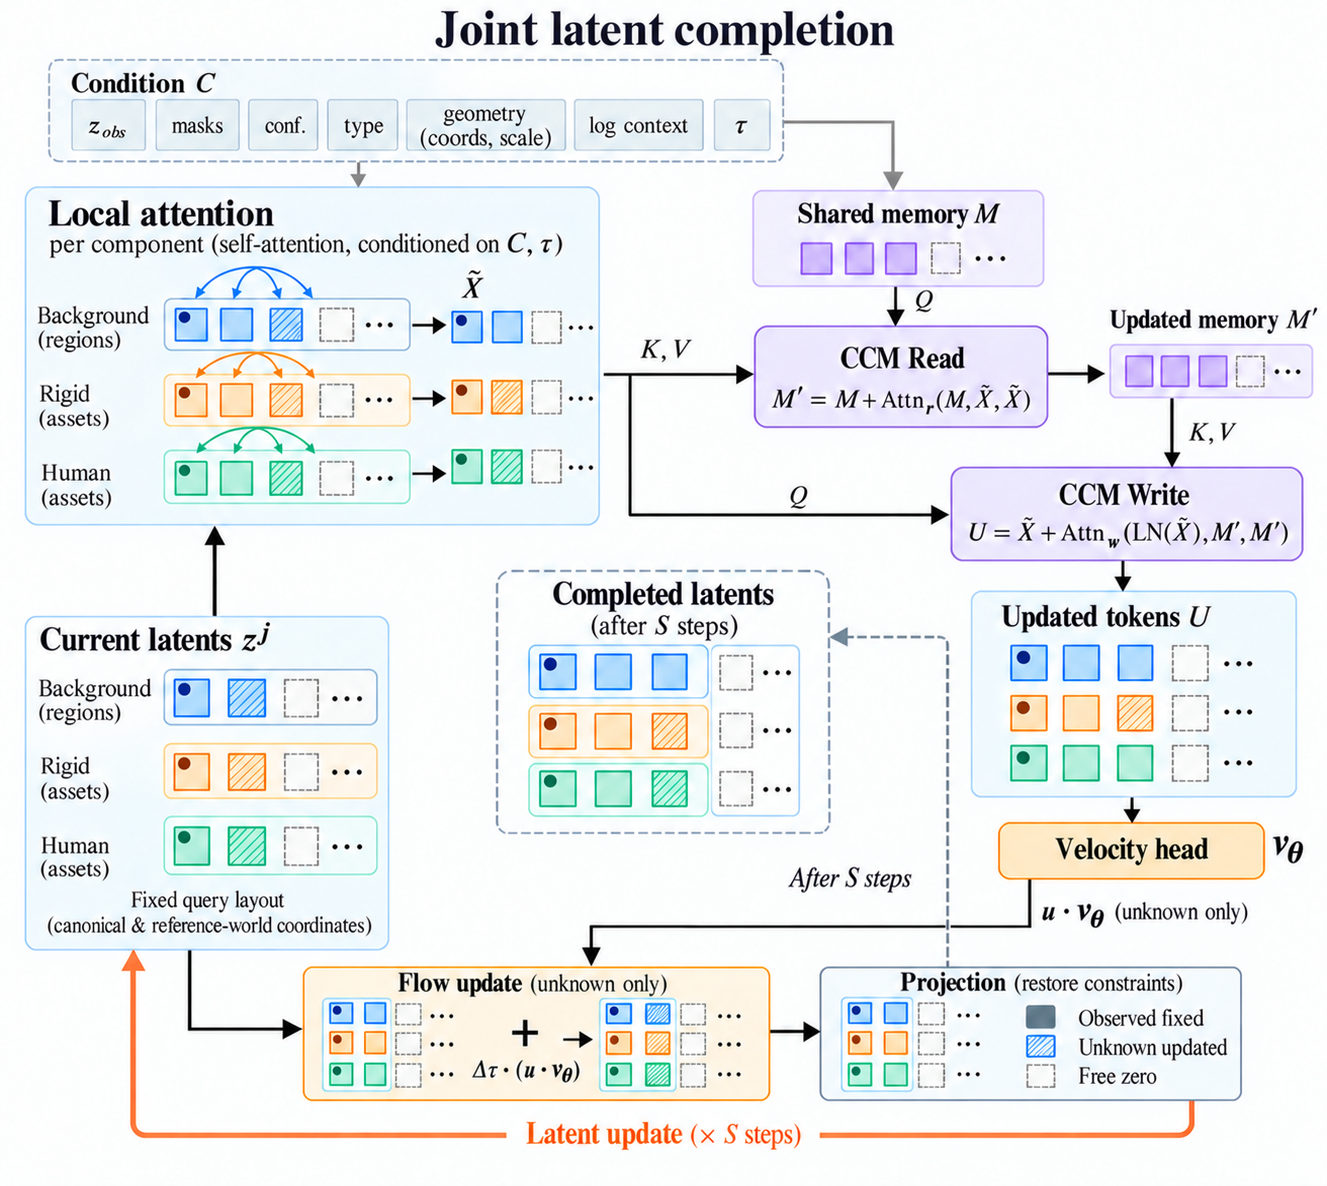
\includegraphics[width=0.86\textwidth]{../fig/drivecompose-joint-completion.png}
\caption{正文联合补全细节图的放大版本。CCM 将组内特征读入共享记忆并写回各组件；速度头与投影更新未知码，同时恢复已见码和清零自由空间码。}
\label{fig:supp-detail}
\end{figure*}

\FloatBarrier
{\small
\bibliographystyle{ieeenat_fullname}
\bibliography{references}
}
\end{document}
